\documentclass[letterpaper,12pt,fleqn]{article}
\usepackage{matharticle}
\usepackage{graphicx}
\usepackage{caption}
\pagestyle{empty}
\begin{document}
\section*{Lab 1: The Natural (Counting) Numbers}

Imagine that you are a hunter-gatherer living prior to 20,000 BC. You only have what you
can carry because you are constantly on the move in order to eat and to avoid being
eaten. You don't accumulate anything, so there is no need to count.

Then, around 20,000 BC, Cro Magnon man starts doing something interesting --- making
marks on bones and sticks. Here is the earliest known example from Central Africa called
the Ishango bone:

\begin{figure}[h]
  \centering
  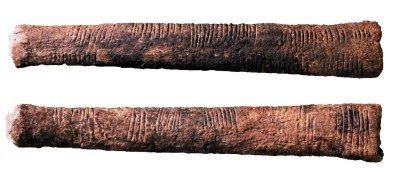
\includegraphics{ishango_bone.jpg}
  \caption*{The Ishango Bone (circa 20,000 BC)}
\end{figure}

Man is counting! This counting coincides with the transition from hunter-gatherer to more
stationary agricultural societies.  What do you think are some of the things that early
man is counting?

This is not a trivial thing. Man is not just pointing to sheep and counting them, he is
making a connection in his mind between the marks on a stick and the animals in the
field.

Today, we do something similar, but instead of marks on a stick, we use numbers. For
counting, we use the familiar Hindu-Arabic number system, invented somewhere between the
$1^{st}$ and $4^{th}$ centuries:
\[1, 2, 3, 4, 5, 6, 7, 8, 9, 10, \ldots\]
We call these the \emph{natural} or \emph{counting} numbers.

Note that the natural numbers start with the number $1$. The three dots at the end are
called an \emph{ellipsis}. This means that the pattern continues in the same fashion.
Where does it stop? If you think about it, given any natural number, you can always add
one to it to get another number. So the answer is that it does not stop. You may have
heard the phrase, ``it goes on until infinity.'' Indeed, infinity, denoted by $\infty$,
is a concept that we will talk about later in the course. The important thing to
remember is that $\infty$ is \emph{not} a number, although it will seem like we treat it
like a number from time to time. Instead, it represents the concept or process of
``keep going and don't stop.'' Thus, we \emph{do not} write something like this:
\[1, 2, 3, 4, 5, \ldots, \infty\hspace{4ex}\mbox{WRONG!}\]

\subsection*{Questions}

\begin{enumerate}
\item List three things that early man may have been counting.

  \vspace{1in}

\item Write the first 20 natural numbers followed by an ellipsis.

  \vspace{1in}

\item Practice writing $\infty$ five times. Make sure that you make the two lobes equal
  size.
  
  \vspace{1in}

\item Indicate whether or not each of the following is a natural number:
  \begin{enumerate}
  \item $5$

    \vspace{0.25in}

  \item $0$

    \vspace{0.25in}

  \item $-1$

    \vspace{0.25in}

  \item $1,000,000$

    \vspace{0.25in}

  \item $\infty$
  \end{enumerate}

\end{enumerate}

\end{document}
